\documentclass[a4]{article}

\usepackage[14pt]{extsizes}
\usepackage[T2A]{fontenc}
\usepackage[utf8]{inputenc}
\usepackage{natbib}
\usepackage{graphicx}
\usepackage[english, russian]{babel}
\usepackage{fontspec}
\usepackage{amsmath}
\usepackage{amsfonts}
\usepackage{amssymb}
\usepackage{amsthm}
\usepackage{mathtools}
\usepackage{mathrsfs}
\usepackage{icomma}
\usepackage{fullpage}
\usepackage{ulem}
\usepackage{eufrak}
\usepackage{setspace}
\usepackage{listings}
\usepackage{indentfirst}
\usepackage[left=2cm,right=1.5cm,top=2cm,bottom=2cm]{geometry}
\usepackage{xcolor}
\usepackage{float}
\usepackage{csquotes}
\usepackage{hyperref}
\usepackage{graphics}



\definecolor{urlcolor}{HTML}{0000FF} % цвет гиперссылок
\definecolor{linkcolor}{HTML}{000000} % цвет гиперссылок
\hypersetup{pdfstartview=FitH, linkcolor=linkcolor, urlcolor=urlcolor, colorlinks=true}


\setmainfont[Ligatures={TeX,Historic}]{Times New Roman}
\setlength{\parindent}{5ex}
\setlength{\parskip}{1em}
\renewcommand{\baselinestretch}{1}

\graphicspath{{images/}}


\definecolor{buzzlightyear}{HTML}{8757A5}
\definecolor{grass}{HTML}{738D06}
\definecolor{literal}{HTML}{F18A2B}
\definecolor{commentcolor}{HTML}{8E908B}

\lstdefinestyle{habrstyle}{
    backgroundcolor=\color{white},
    commentstyle=\color{commentcolor},
    keywordstyle=\bfseries\color{buzzlightyear},
    numberstyle=\tiny\color{commentcolor},
    stringstyle=\color{grass},
    basicstyle=\ttfamily\footnotesize,
    breakatwhitespace=false,
    breaklines=true,
    captionpos=b,
    keepspaces=true,
    numbers=left,
    numbersep=5pt,
    showspaces=false,
    showstringspaces=false,
    showtabs=false,
    tabsize=4
}

\lstset{style=habrstyle}

\begin{document}
    % НАЧАЛО ТИТУЛЬНОГО ЛИСТА
    \begin{center}
        \begin{center}
            \hfill \break
            \normalsize{Санкт-Петербургский государственный политехнический}\\
            \normalsize{университет Петра Великого}\\
            \hfill \break
            \normalsize{\textbf{Высшая школа интеллектуальных систем и}}\\
            \normalsize{\textbf{суперкомпьютерных технологий}}\\
            \hfill \break
            \hfill \break
            \hfill \break
            \normalsize{Лабораторная работа}\\
            \hfill \break
            \normalsize{\LARGE Сигналы и звуки}\\
        \end{center}
        \hfill \break
        \hfill \break
        \hfill \break
        \hfill \break
        \hfill \break
        \hfill \break
        \hfill \break
        \hfill \break
        \hfill \break
        \hfill \break
        \begin{tabbing}
            Выполнил студент гр. 3530901/80201 \`И.С. Иванов\\
            \\
            Преподаватель: \`Н.В. Богач\\
        \end{tabbing}
        \hfill \break
        \hfill \break
        \hfill \break
        \hfill \break
        \begin{center}
            Санкт-Петербург\\
            2021
        \end{center}
        \thispagestyle{empty}
    \end{center}
    % КОНЕЦ ТИТУЛЬНОГО ЛИСТА

    % ОГЛАВЛЕНИЕ
    \newpage
    \tableofcontents

    % СПИСОК ИЛЛЮСТРАЦИЙ
    \newpage
    \listoffigures

    % СПИСОК ЛИСТИНГОВ
    \newpage
    \lstlistoflistings

    \newpage


    \section{Упражнение №1: Изучить примеры из chap01}
    \label{sec:1_study_examples}

    Для выполнения первого пункта необходимо изучить и выполнить примеры из файла chap01.ipynb.
    Запустим все примеры из этого файла.

    \begin{figure}[h]
        \centering
        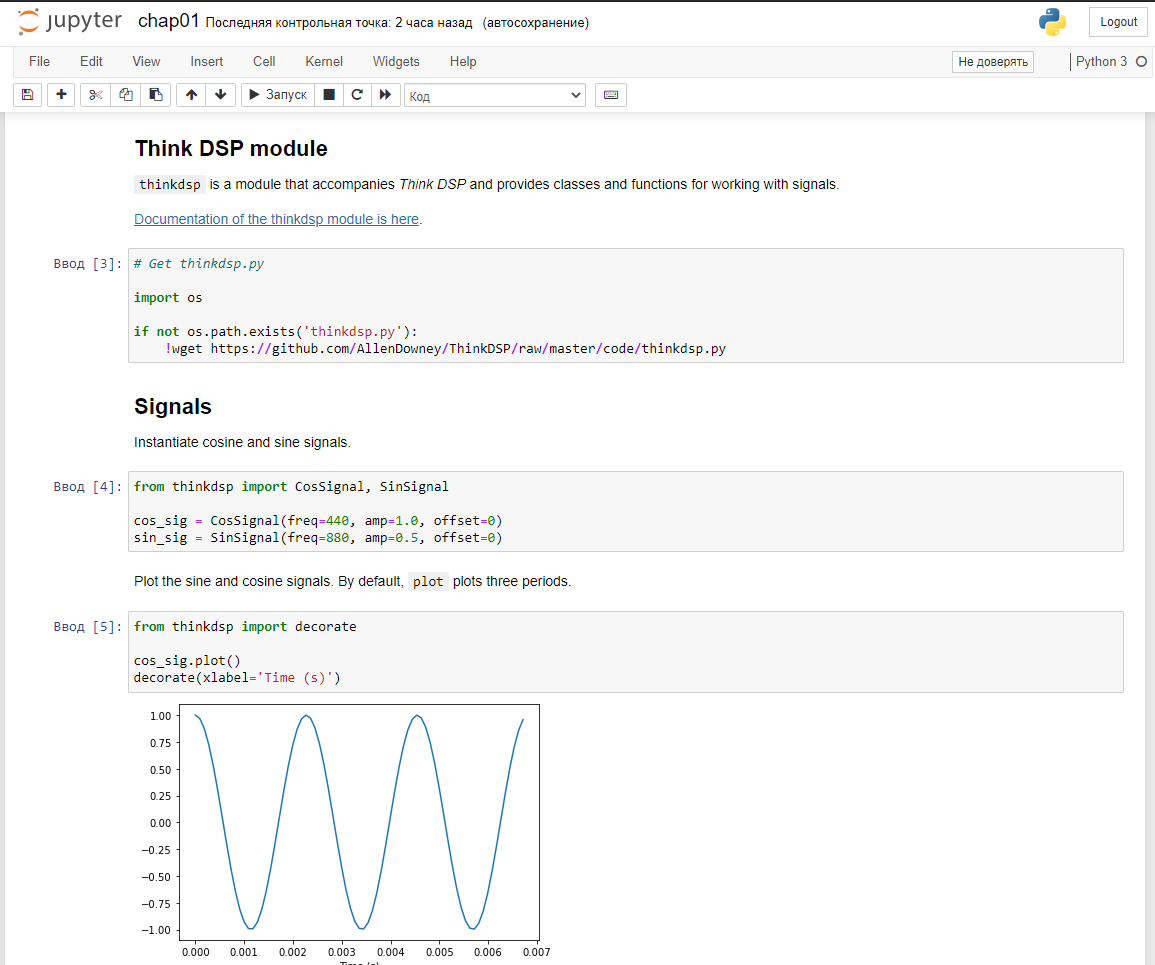
\includegraphics[width=\textwidth]{1}
        \caption{Изучение и проверка примеров из файла (1)}
        \label{fig:check_it_works_1}
    \end{figure}

    \begin{figure}[h]
        \centering
        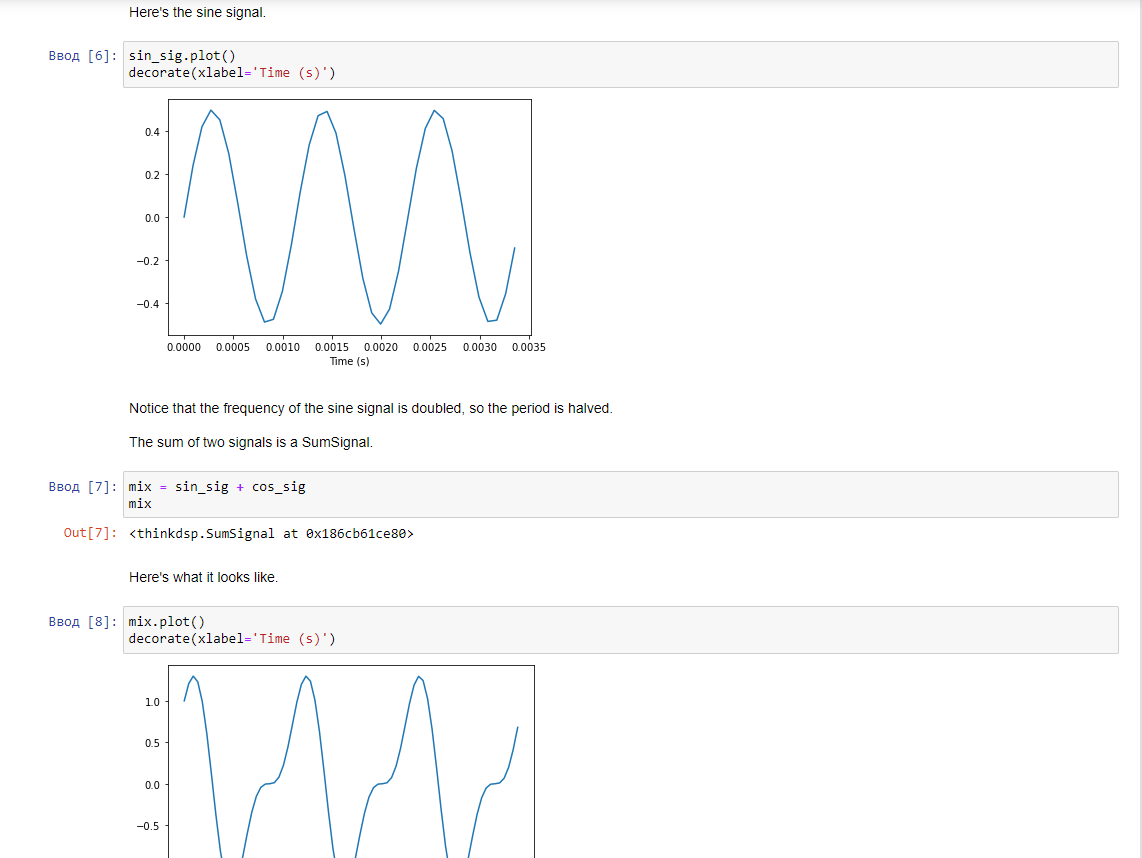
\includegraphics[width=\textwidth]{2}
        \caption{Изучение и проверка примеров из файла (2)}
        \label{fig:check_it_works_2}
    \end{figure}

    \newpage


    \section{Упражнение №2: Обработка сигналов}
    \label{sec:2_signal_processing}

    Во втором упражнении необходимо сначала скачать с сайта \href{https://freesound.org/}{https://freesound.org/} любой образец звука, имеющий четко выраженную высоту и выделить в нем полусекундный фрагмент с постоянной высотой.
    Необходимо вычислить и рассчитать спектр выбранного фрагмента.
    Далее нужно произвести фильтрацию гармоник и преобразовать спектры обратно в сигнал.

    Необходимо проверить наличие файла \texttt{thinkdsp.py} и скачать его при отсутствии:

    \begin{lstlisting}[language=Python, caption= Проверка наличия \texttt{thinkdsp.py}, label={lst:check_thinkdsp}]
        import os
        if not os.path.exists('thinkdsp.py'):
            from urllib.request import urlretrieve
            urlretrieve("https://github.com/AllenDowney/ThinkDSP/raw/master/code/thinkdsp.py", "thinkdsp.py")
    \end{lstlisting}

    Далее импортируем из раннее проверенного файла функции, и прочитаем файл с образцом звука:

    \begin{lstlisting}[language=Python, caption= Чтение скаченного образца звука, label={lst:read_wav}]
        from thinkdsp import read_wave
        wave = read_wave('Sounds/105384__drzoom__hitting-pan-top-large.wav')
        wave.normalize()
        wave.make_audio()
    \end{lstlisting}

    После чтения образца звука выведем график:

    \begin{lstlisting}[language=Python, caption= Вывод графика образца,label={lst:wav_plot}]
        wave.plot()
    \end{lstlisting}

    \begin{figure}[H]
        \centering
        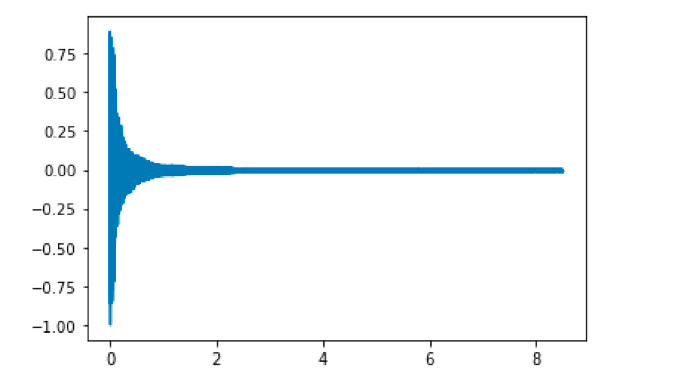
\includegraphics[width=\textwidth]{wav_plot_1}
        \caption{График образца звука}
        \label{fig:plot_wav_1}
    \end{figure}

    Далее необходимо выбрать сегмент из нашего образца звука.
    Был взят сегмент от нулевой секунды длительностью 0.3 секунды:

    \begin{lstlisting}[language=Python, caption= Выбор сегмента, label={lst:segment_choose}]
        segment = wave.segment(start=0, duration=0.3)
        segment.make_audio()
    \end{lstlisting}

    Теперь выведем график на экран:

    \begin{lstlisting}[language=Python, caption= Вывод графика, label={lst:segment_plot}]
        segment.plot()
    \end{lstlisting}

    \begin{figure}[H]
        \centering
        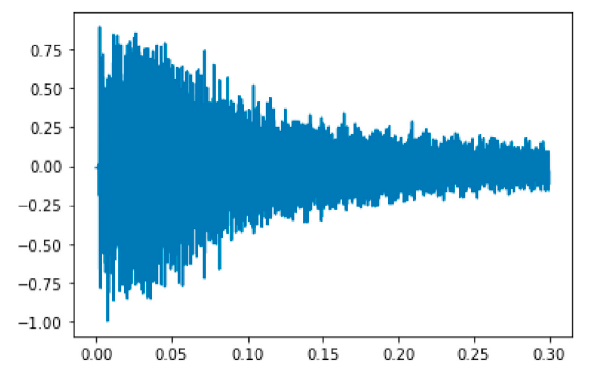
\includegraphics[width=\textwidth]{segment_plot}
        \caption{График сегмента}
        \label{fig:plot_segment_1}
    \end{figure}

    После этого посмотрим как выглядит наш спектр:

    \begin{lstlisting}[language=Python, caption= Изображение спектра, label={lst:spectr_segment}]
        spectrum = segment.make_spectrum()
        spectrum.plot(high=7000)
    \end{lstlisting}

    \begin{figure}[H]
        \centering
        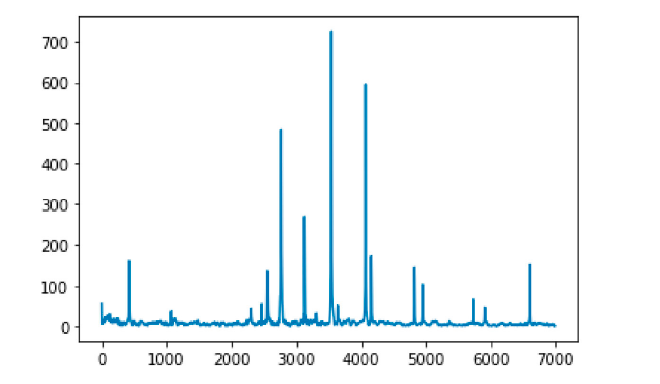
\includegraphics[width=\textwidth]{segment_spectr}
        \caption{Изображение спектра}
        \label{fig:segment_spectr}
    \end{figure}

    Увеличим спектр

    \begin{lstlisting}[language=Python, caption= Приближенное изображение спектра, label={lst:zoom_spectr}]
        spectrum = segment.make_spectrum()
        spectrum.plot(high=4500)
    \end{lstlisting}

    \begin{figure}[H]
        \centering
        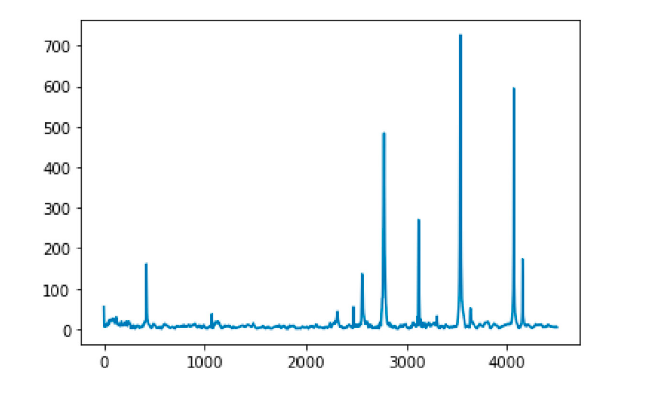
\includegraphics[width=\textwidth]{zoomed_spectr}
        \caption{Увеличенное изображение спектра}
        \label{fig:zoomed_spectr}
    \end{figure}

    Далее, фильтрация спектра:

    \begin{lstlisting}[language=Python, caption= Фильтрация спектра, label={lst:filter_spectr}]
        spectrum.low_pass(2000)
        spectrum.plot(high=4000)
    \end{lstlisting}

    Далее вывод графика отфильтрованного спектра:

    \begin{figure}[H]
        \centering
        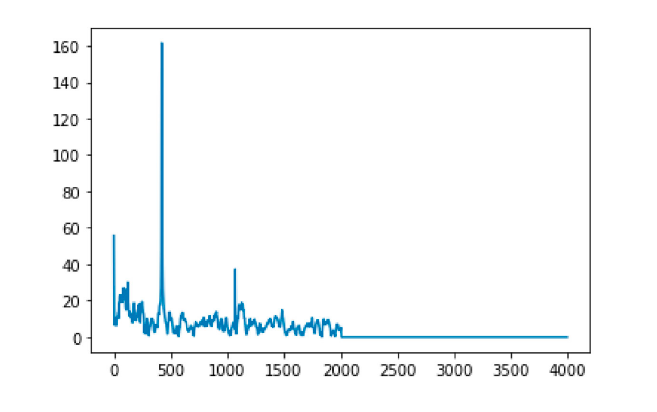
\includegraphics[width=\textwidth]{filtered_spectr}
        \caption{Отфильтрованный спектр}
        \label{fig:spectr_filter}
    \end{figure}

    Переводи отфильтрованный спектр обратно в аудио:

    \begin{lstlisting}[language=Python, caption= Перевод в аудио, label={lst:spectr_to_wav}]
        spectrum.make_wave().make_audio()
    \end{lstlisting}

    По результатам выполнения данного упражнения можно сделать вывод, что в полученном звуке отсутствуют частоты выше 2000 Гц.
    Звук стал похожим на звук из низкокачественного динамика.

    \newpage


    \section{Упражнение №3: Сложение сигналов}
    \label{sec:3_sum_signal}
    В третьем упражнении нам необходимо создать сложный сигнал из объектов \texttt{SinSignal} и \texttt{CosSignal} суммируя их.
    Также следует обработать полученный сигнал для получения wave, прослушать его, вычислить для него \texttt{Spectrum} и после вывести на экран.

    \begin{lstlisting}[language=Python, caption= Создание сигналов, label={lst:gen_signal}]
        from thinkdsp import SinSignal, CosSignal

        sin_signal = (SinSignal(freq=400, amp=1.0) +
                  SinSignal(freq=600, amp=0.5) +
                  SinSignal(freq=800, amp=0.25))

        cos_signal = (CosSignal(freq=400, amp=1.0) +
                  CosSignal(freq=600, amp=0.5) +
                  CosSignal(freq=800, amp=0.25))

        sin_signal.plot()
        cos_signal.plot()
    \end{lstlisting}

    В результате получился такой вывод на экран:

    \begin{figure}[H]
        \centering
        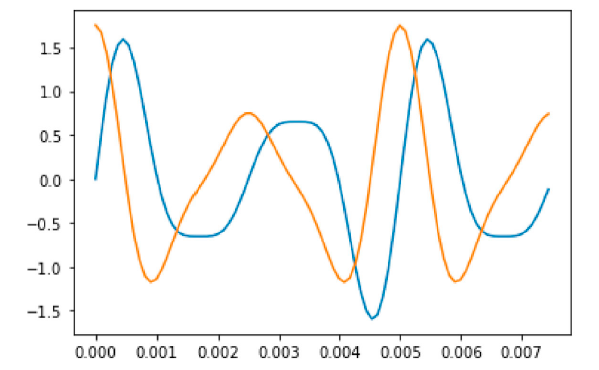
\includegraphics[width=\textwidth]{signals}
        \caption{График сигналов}
        \label{fig:signals}
    \end{figure}

    Теперь сложим два канала и выведем полученный график:

    \begin{lstlisting}[language=Python, caption= Суммирование каналов, label={lst:sum_signal}]
        signal = sin_signal + cos_signal
        signal.plot()
    \end{lstlisting}

    \begin{figure}[H]
        \centering
        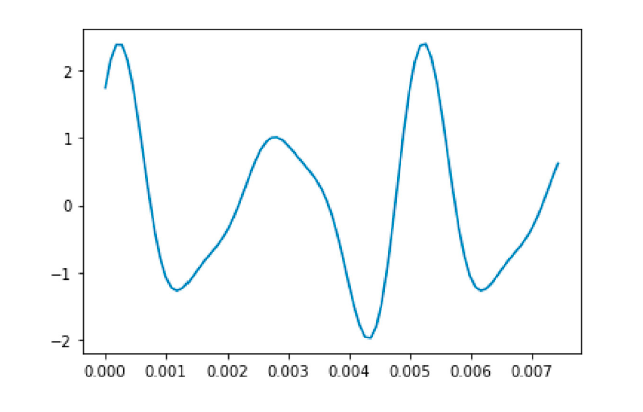
\includegraphics[width=\textwidth]{sum_signals}
        \caption{Суммированный сигнал}
        \label{fig:sum_signals}
    \end{figure}

    После этого было получено аудио из данного сигнала:

    \begin{lstlisting}[language=Python, caption= Получение аудио, label={lst:make_audio_from_signals}]
        wave2 = signal.make_wave(duration=0.5)
        wave2.make_audio()
    \end{lstlisting}

    Получим спектр из полученного сигнала:

    \begin{lstlisting}[language=Python, caption= Получение спектра, label={lst:make_spectr_from_signal}]
        spectrum2 = wave2.make_spectrum()
        spectrum2.plot(high=1000)
    \end{lstlisting}

    \begin{figure}[H]
        \centering
        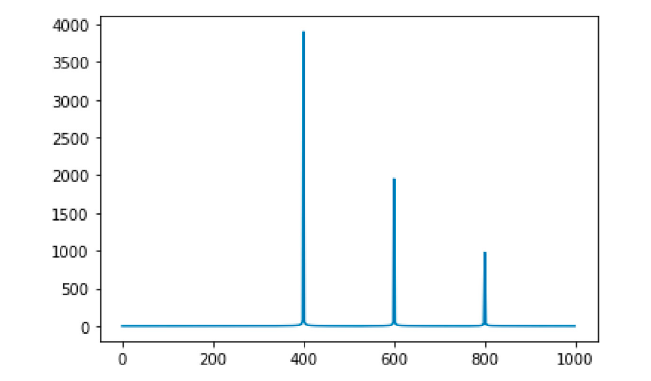
\includegraphics[width=\textwidth]{spectr_signals}
        \caption{Полученный спектр}
        \label{fig:spectr_signals}
    \end{figure}

    Добавим к сигналу синусоидальный сигнал с частотой \texttt{133 Hz} и переведем в аудио:

    \begin{lstlisting}[language=Python, caption= Получение спектра, label={lst:add_sin_133}]
        signal += SinSignal(freq=133, amp=0.75)
        wave3 = signal.make_wave()
        wave3.make_audio()
    \end{lstlisting}

    Получим спектр из сигнала:

    \begin{lstlisting}[language=Python, caption= Полученый спектр, label={lst:spectr_133}]
        wave3.apodize()
        spectrum3 = wave3.make_spectrum()
        spectrum3.plot(high=1000)
    \end{lstlisting}

    \begin{figure}[H]
        \centering
        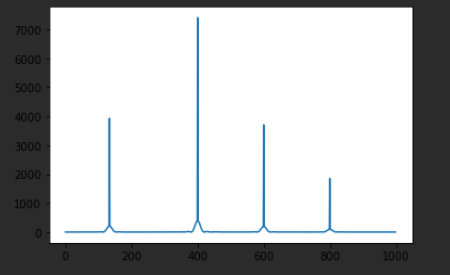
\includegraphics[width=\textwidth]{spectr_133}
        \caption{Полученный спектр}
        \label{fig:spectr_133}
    \end{figure}

    По результатам выполнения данного упражнения можно сделать вывод, что в полученном в конце звуке появились колебания.

    \newpage


    \section{Упражнение №4: Изменение длительности сигнала}
    \label{sec:4_stretch}
    В четвертом упражнении необходимо реализовать функцию \texttt{stretch}, которая принимает сигнал и коэффициент изменения, после чего в зависимости от коэффициента либо замедляет, либо ускоряет сигнал посредством изменения \texttt{ts} и \texttt{framerate}.

    Напишем саму функцию \texttt{stretch}:

    \begin{lstlisting}[language=Python, caption= Функция \texttt{stretch}, label={lst:stretch}]
        def stretch(wav, factor):
            wav.ts *= factor
            wav.framerate /= factor
    \end{lstlisting}

    Прочитаем раннее скачанный звуковой файл:

    \begin{lstlisting}[language=Python, caption= Чтение файла, label={lst:load_wave4}]
        wave4 = read_wave('Sounds/105384__drzoom__hitting-pan-top-large.wav')
        wave4.normalize()
        wave4.make_audio()
    \end{lstlisting}

    Вызов функции \texttt{stretch}.
    Параметры wav = wave4 и factor = 0.5, затем получим аудио:

    \begin{lstlisting}[language=Python, caption= Вызов функции \texttt{stretch},label={lst:stretch_call}]
        stretch(wave4, 0.5)
        wave4.make_audio()
    \end{lstlisting}

    Спектр полученной дорожки:

    \begin{lstlisting}[language=Python, caption= Спектр после вызова функции \texttt{stretch}, label={lst:get_spectr}]
        wave4.plot()
    \end{lstlisting}

    \begin{figure}[H]
        \centering
        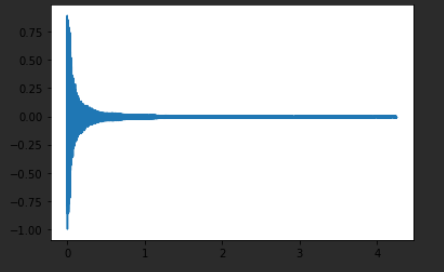
\includegraphics[width=\textwidth]{stretch_audio_result}
        \caption{Спектр аудиодорожки}
        \label{fig:stretch_audio_result}
    \end{figure}

    По результатам выполнения данного упражнения можно сделать вывод, что полученная функция \texttt{stretch} действительно замедляет или ускоряет полученный сигнал.

    \newpage


    \section{Выводы}
    \label{sec:conclusions}
    В результате выполнения данной лабораторной работы мы изучили как надо работать с сигналами, как их обрабатывать, фильтровать и воспроизводить из с помощью библиотеки Python.
    Кроме того была реализована и проверена функция для преобразования полученного сигнала.
    Также нами были получены сведения об основных понятиях и навыки работы с сигналами.

\end{document}